\makeatletter
\def\@seccntformat#1{\csname #1ignore\expandafter\endcsname\csname the#1\endcsname\quad}
\renewcommand{\@seccntformat}[1]{}
\let\sectionignore\@gobbletwo
\let\latex@numberline\numberline
\def\numberline#1{\if\relax#1\relax\else\latex@numberline{#1}\fi}
\makeatother

\onlyifstandalone{
\setcounter{page}{1}
\setcounter{section}{0}
\renewcommand{\thetable}{S\arabic{table}}

\setcounter{figure}{0}
\renewcommand{\thefigure}{S\arabic{figure}}
}

\doublespacing

\onlyifstandalone{
\begin{refsection}
}

\section{Methodological Supplement}\label{ch04:appendix}
\onlyifstandalone{
\setcounter{section}{0}
}

The code to reproduce our models, analyses, and plots is available at \url{https://github.com/sdaza/dissertation/tree/master/ch04}. In this supplement, we show and discuss the verification and calibration of MIA's modules to ensure our model implementation is correct. For this purpose, MIA's general setup is: (a) 30 counties with an initial population of 100 agents, (b) five income groups (quintiles), (c) a population limit per county of 10\% the expected population at time $t$, (d) a decision moving rate of $mob_r = 0.10$, (e) 30 replicates per scenario, and (f) 30 as the the last complete generation before finishing the simulation.

\subsection{Demographic dynamics}\label{ch04:appendix_demographics}

To examine MIA's demographic behavior, we collected individual information for generations 20, 25, and 30, over 30 replicates. Figure \ref{ch04:population_verification} summarizes the key demographic processes implemented in MIA using US mortality and fertility rates as baselines (Table \ref{ch04:rates}). We adjusted fertility rates to create a relatively stable population and keep the size of income groups relatively even (e.g, the lowest income group has a higher mortality rate, but also a higher fertility rate relative to the highest income group). As expected, the average number of offsprings per agent is practically 1. The distribution of age of death follows the shape expected given the age-specific mortality rates in the US, with an upper cut-off at 110 years (all agents must die by age 110). There are picks of mortality at the beginning of each 5-year age interval. This is expected as the timing is sampled from an exponential distribution when an agent enters an age group. Simulated life expectancy for complete cohorts concentrates around 76.3 years, close to 78.6, the life expectancy estimated by \citet{kochanek2019} for the US (2017). The life expectancy values are not the same as the ones estimated by \citet{kochanek2019} because the baseline mortality rate is not adjusted by income and the exposure to the county's conditions or income-specific effects that modify the mortality risk in groups of agents.\footnote{When all income effects on mortality and smoking are removed, the estimated life expectancy is 78.4, practically the same as the life expectancy estimation reported by \citet{kochanek2019}.} The population sizes are relatively stable and uniform overtime, although the total number of agents fluctuates considerably by replicate. The differences in life expectancy by income group are in the same order of magnitude as the differences reported by \citet{chetty2016}: around seven years between the highest and lowest quintile when income-specific effects on smoking and mortality are active.

\renewcommand{\arraystretch}{1.0}
% results table
\begin{table}[htp]
\centering
\begin{threeparttable}
\setlength{\tabcolsep}{30pt}
\footnotesize
\caption{Mortality and fertility rates} \label{ch04:rates}
\begin{tabular}{llrr}
\hline
\addlinespace
Age group	& Mortality rate$^1$  & Fertility rate$^2$  \\
%& Smoking initiation rate$^2$ \\
\addlinespace
\hline
\addlinespace
0	& 567.0	    & 0	     \\
1	& 24.3	    & 0	     \\
5	& 11.6	    & 0	     \\
10	& 15.5	    & 0.2    \\
15	& 51.5	    & 17.4	 \\
% 18	& 51.5	    & 17.4	 \\
20	& 95.6	    & 68.0	 \\
25	& 121.0	    & 95.3	 \\
30	& 145.4	    & 99.7	 \\
35	& 173.8	    & 52.6	 \\
40	& 218.4	    & 11.8	 \\
45	& 313.2	    & 0.9	 \\
50	& 488.0	    & 0	     \\
55	& 736.5	    & 0	     \\
60	& 1050.2	& 0	     \\
65	& 1473.5	& 0	     \\
70	& 2206.9	& 0	     \\
75	& 3517.8	& 0	     \\
80	& 5871.7	& 0	     \\
85	& 13573.6	& 0	     \\
\addlinespace
\hline
\addlinespace
\end{tabular}
   \begin{tablenotes}
      \scriptsize
       \item[1] Rates are per 100,000 population in the US \citep[Table 2, pg. 24]{kochanek2019}.
       \item[2] Rates are births per 1,000 women in the US \citep[Table 2, pg. 13]{martin2019}.
    %   \item[3] Smoking initiation rates in New Zealand \citep{edwards2013}.
    \end{tablenotes}
  \end{threeparttable}
\end{table}

\newpage
\begin{figure}[htp]
    \caption{Population Dynamics (30 replicates)}\vspace{5mm}
    \label{ch04:population_verification}
     \centering
     \begin{subfigure}[b]{0.4\textwidth}
        %\caption{Number of kids}
         \centering
         \includegraphics[width=\textwidth]{plots/verification/population/num_kids.pdf}
     \end{subfigure}
    %  \hfill
     \begin{subfigure}[b]{0.4\textwidth}
        %\caption{Age of death}
         \centering
         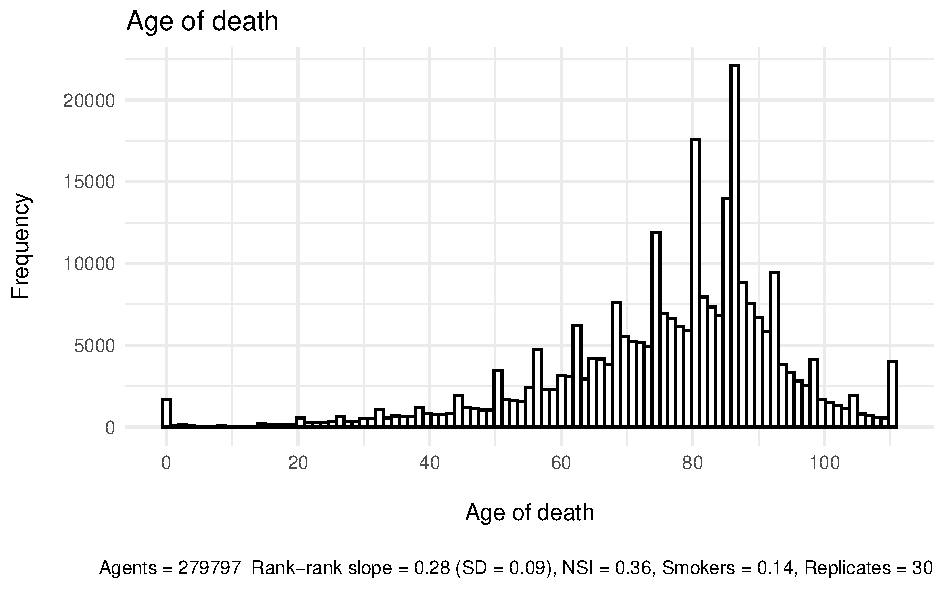
\includegraphics[width=\textwidth]{plots/verification/population/age_death.pdf}
     \end{subfigure}\vspace{5mm}

     \begin{subfigure}[b]{0.4\textwidth}
         %\caption{Life expectancy}
         \centering
         \includegraphics[width=\textwidth]{plots/verification/population/le.pdf}
     \end{subfigure} %
     \begin{subfigure}[b]{0.4\textwidth}
        %\caption{Population size}
         \centering
         \includegraphics[width=\textwidth]{plots/verification/population/population.pdf}
     \end{subfigure}
\end{figure}


\subsection{Residential mobility and segregation}\label{ch04:appendix_segregation}

The segregation mechanism is an adaptation of Schelling's segregation model \citep{schelling2006}. Agents live in counties and at rate $mob_r$ decide whether to move or stay in the current county. With a probability $mob_{rand}$, agents decide to move to new county either randomly or based on the proportion of people with the same income group living in a county and similarity tolerance threshold $mob_{thr}$. Suppose the proportion of people in the income group $k$ is lower than the tolerance threshold $mob_{thr}$. In that case, agents would move to a random county, excluding those that have reached their population limit so that to avoid an extreme concentration of agents in only some counties. Figure \ref{ch04:action_chart_residential_mobility} displays the decision chart associated with the residential mobility mechanism.

\newpage
\begin{figure}[htp]
    \caption{Agent's decision chart for residential mobility} \label{ch04:action_chart_residential_mobility}
    \centering
    % \frame{
        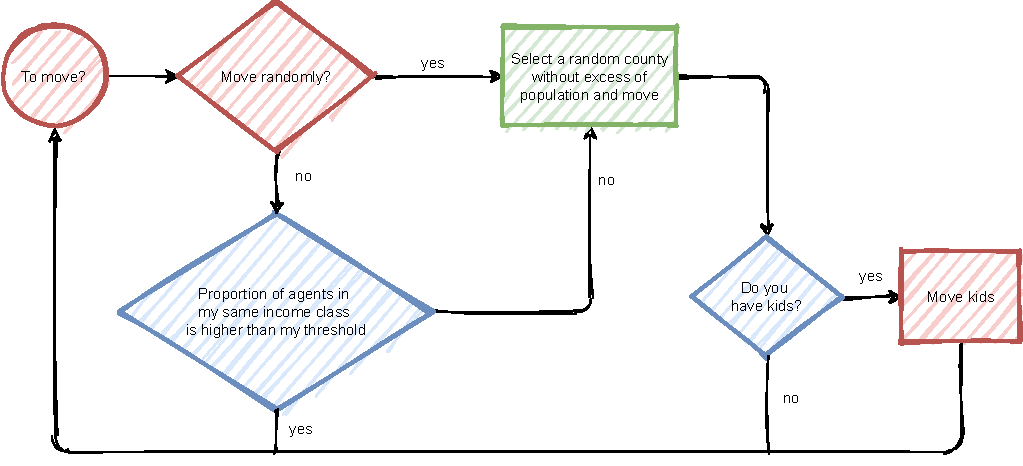
\includegraphics[scale=0.8]{plots/action-chart-residential-mobility.pdf}
    % }
\end{figure}

We use the neighborhood sorting index or NSI to measure income segregation \citep{jargowsky2005}. The NSI compares the income variation across all neighborhoods (or counties) in a metro area with the income variation across all households in that metro area. If agents are segregated across counties by income, the income variation across counties will be similar to the income variation across agents, and the NSI will equal almost 1. If all counties are perfectly economically integrated (i.e., each county is a microcosm of the entire population), the NSI will be almost 0.

Thus, the NSI is a measure of the neighborhood's heterogeneity, normalized by income variance. It measures segregation by showing how much aggregating data lose information about variation in individual income. However, it fails to capture larger-scale features of neighborhoods' spatial arrangement. The NSI is not affected if all high-income neighborhoods are clustered in one part of the metropolitan area or scattered randomly around the map. For the propose of our model, that limitation is not problematic.

To examine the changes in the levels of income segregation, we use a decision to move rate ($mob_r$) of 0.10 per year. When movement is completely random, that rate generates  about 7.6 moves on average over agents' life course. Once the segregation mechanism is in action, the number of moves is reduced about half as agents do not always have incentives to leave their county of residence. We explored three scenarios: (1) all agents move randomly, (2) only 1\% of agents move randomly with tolerance threshold 0.15, and (3) we increased the tolerance threshold to 0.22. Figure \ref{ch04:segregation_verification} shows the dynamics of the NSI over 30 simulated generations and about 1100 simulation years per replicate. The NSI goes from 0.07 when the movement is completely random, to 0.36 when the moving threshold is 0.22. 

\begin{figure}[htp]
    \caption{Neighborhood sorting index (NSI) by year (30 replicates)}\vspace{5mm}
    \label{ch04:segregation_verification}
     \centering
     \begin{subfigure}[b]{0.50\textwidth}
         \centering
         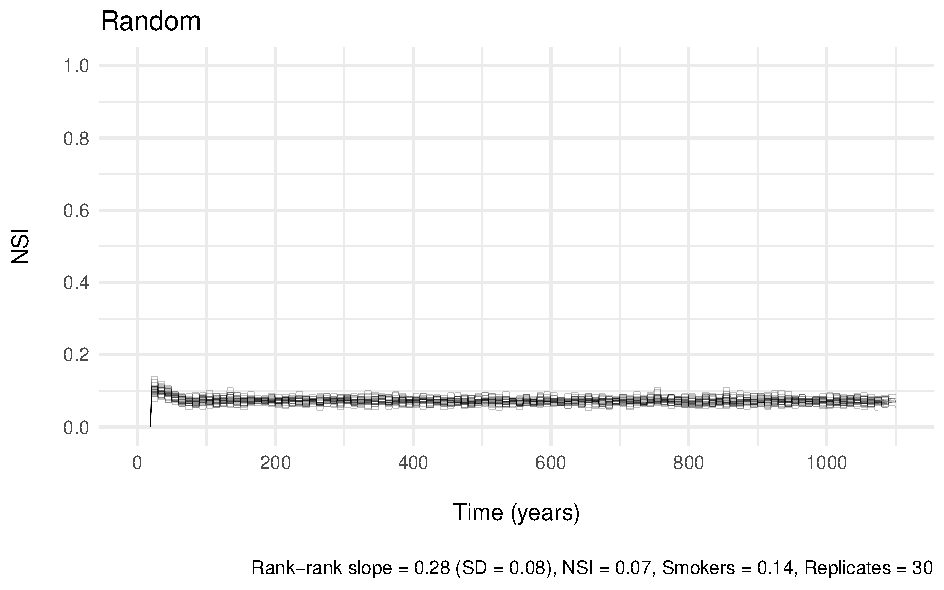
\includegraphics[width=\textwidth]{plots/verification/segregation/nsi_4.pdf}
     \end{subfigure}%
     \begin{subfigure}[b]{0.50\textwidth}
         \centering
         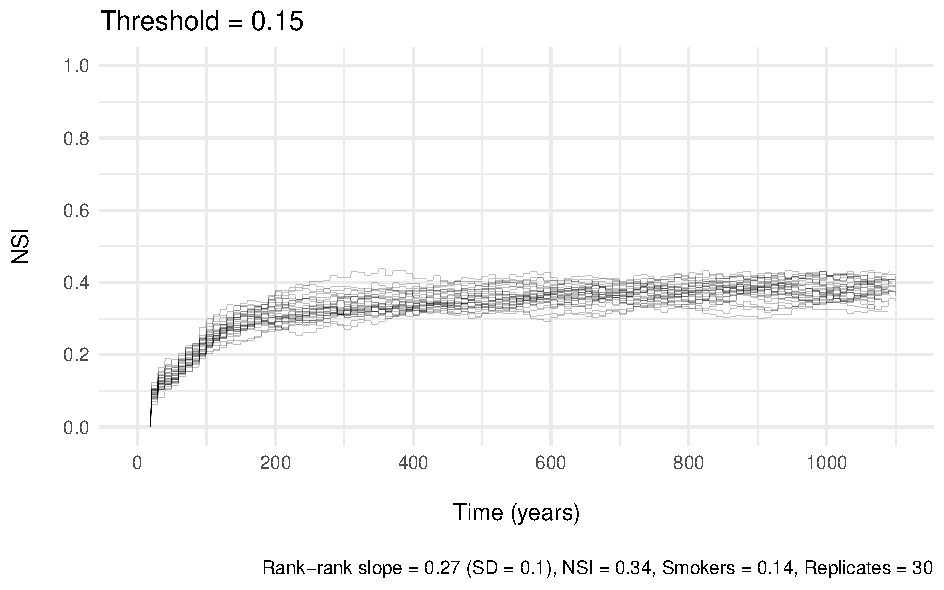
\includegraphics[width=\textwidth]{plots/verification/segregation/nsi_1.pdf}
     \end{subfigure}\vspace{7mm}

     \begin{subfigure}[b]{0.50\textwidth}
         \centering
         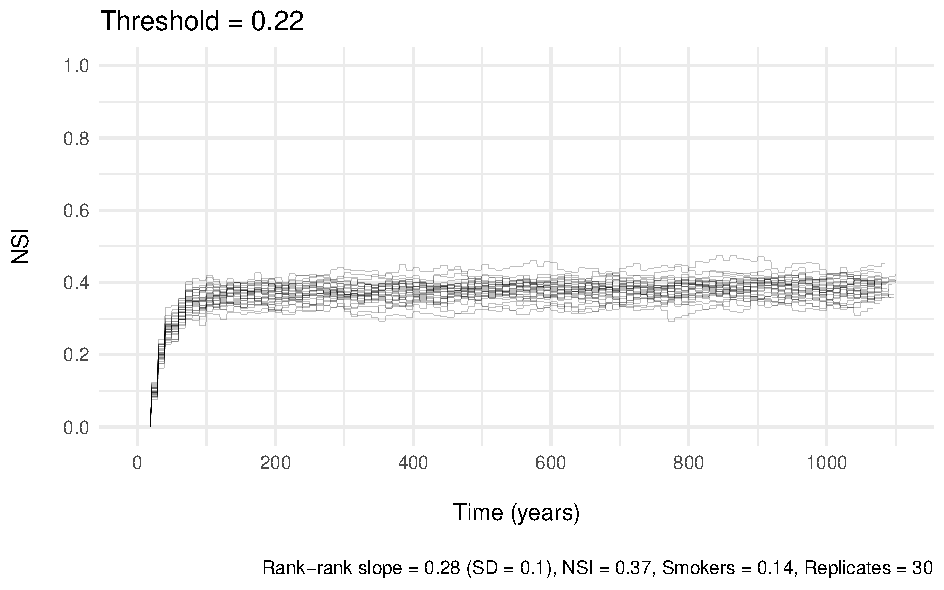
\includegraphics[width=\textwidth]{plots/verification/segregation/nsi_2.pdf}
     \end{subfigure} %
    %  \begin{subfigure}[b]{0.4\textwidth}
    %      \centering
    %      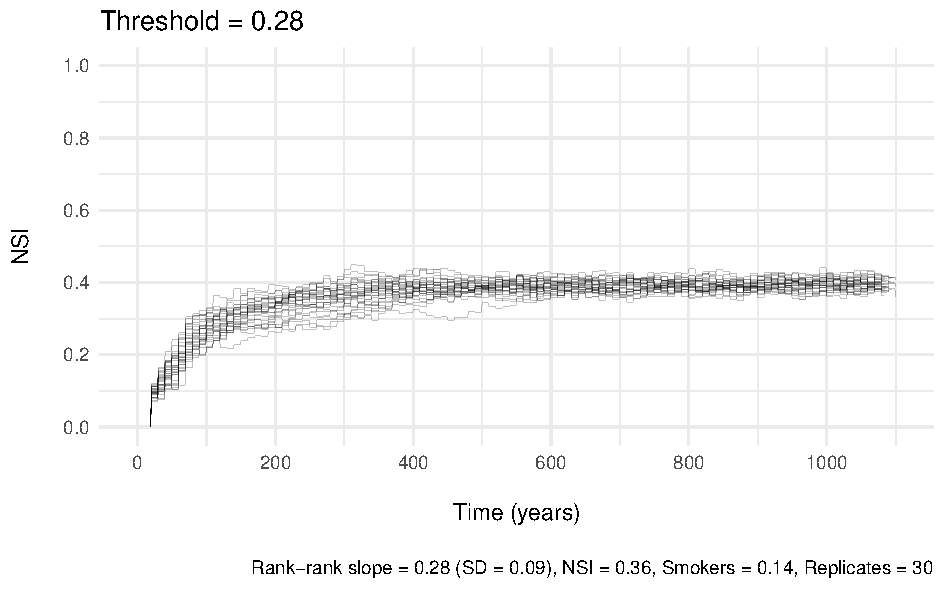
\includegraphics[width=\textwidth]{plots/verification/segregation/nsi_3.pdf}
    %  \end{subfigure}

\end{figure}


These differences depend on how the segregation model was implemented (income transition matrices used, number of income groups and counties). Despite random fluctuations, the NSI trajectories are relatively stable over time. As expected, the highest number of moves is observed when the movement is completely random (7.6 moves on average during  agents' life course), while the fewest moves (0.7) when $mob_{thr}$ is the lowest (0.15), and 2.3 moves when $mob_{thr} = 0.22$. The average of moves during childhood (before age 18) goes from 0.25 to 1.8. According to \citet{jargowsky2017}, the economic segregation in the US in 2010 was 0.396. To reproduce those levels of income segregation, we use a tolerance threshold $mob_{thr}$ that generates NSI levels close to 0.40.

%\footnote{When the moving rate $mob_r$ is 0.10, the average number of moves per agent is around six, and practically all agents (97\%) change to a different county at least once in life.}.

%   niteration prob_move_random                 move_threshold        nsi     N
% 1:          1             0.01 [0.15, 0.15, 0.15, 0.15, 0.15] 0.33327856 32778
% 2:          2             0.01 [0.22, 0.22, 0.22, 0.22, 0.22] 0.36385852 32601
% 3:          3             0.01 [0.28, 0.28, 0.28, 0.28, 0.28] 0.35514859 32653
% 4:          4             1.00      [0.1, 0.1, 0.1, 0.1, 0.1] 0.07159594 32714
%           sd      prop
% 1: 0.07836195 0.2351245
% 2: 0.06544093 0.1798527
% 3: 0.07883175 0.2219683
% 4: 0.01422140 0.1986342

%   niteration prob_move_random                 move_threshold     moves
% 1:          4             1.00      [0.1, 0.1, 0.1, 0.1, 0.1] 7.6680209
% 2:          1             0.01 [0.15, 0.15, 0.15, 0.15, 0.15] 0.7237324
% 3:          2             0.01 [0.22, 0.22, 0.22, 0.22, 0.22] 2.3017078
% 4:          3             0.01 [0.28, 0.28, 0.28, 0.28, 0.28] 3.5267212
%   moves_kid
% 1: 1.7746925
% 2: 0.2572882
% 3: 0.6537245
% 4: 0.9532554

% Given the number of income groups, a higher moving threshold would make it more difficult to satisfy the agent's threshold and increase the agent's movement, not producing income segregation.

\subsection{Income mobility}

MIA's income generation and mobility mechanisms consist of two components: (1) the link between the parent's and child's income group, and (2) the impact of the exposure to the county's resources on child's income group. We verified the implementation of both mechanisms by examining the distribution of income, income mobility, and segregation. We defined three scenarios or iterations using the baseline parameters (see Table \ref{ch04:abm_parameters} in the paper): (1) the base probability of being in the same income group of the parent is 0.30, the probability for the rest of the income groups is $(1 - 0.3)/4 = 0.175$, and $w_k = 0$, that is, there is no effect of the county's income group composition on the child's income group definition; (2) the same as (1), but this time the transition probabilities change based on the exposure of county income group composition using ($w_k = 0.5$); (3) the transition probabilities come from a sample of commuting zones probabilities estimated by \citet{chetty2014}, and they are assigned at the county level using $w_k = 0$. As expected, MIA generates an income distribution that mimics the IPUMS family income distribution (sample size = 250,000, see Figure \ref{ch04:income_distribution}). Once an agent has been assigned to an income class (1 to 5), we drew a weighted-sample from the IPUMS income distribution for that income quintile. 

\vspace{5mm}
\begin{figure}[htp]
    \caption{Individual income distribution (30 replicates)}\vspace{5mm}
    \label{ch04:income_distribution}
     \centering
     \begin{subfigure}[b]{0.45\textwidth}
        % \caption{Number of kids}
         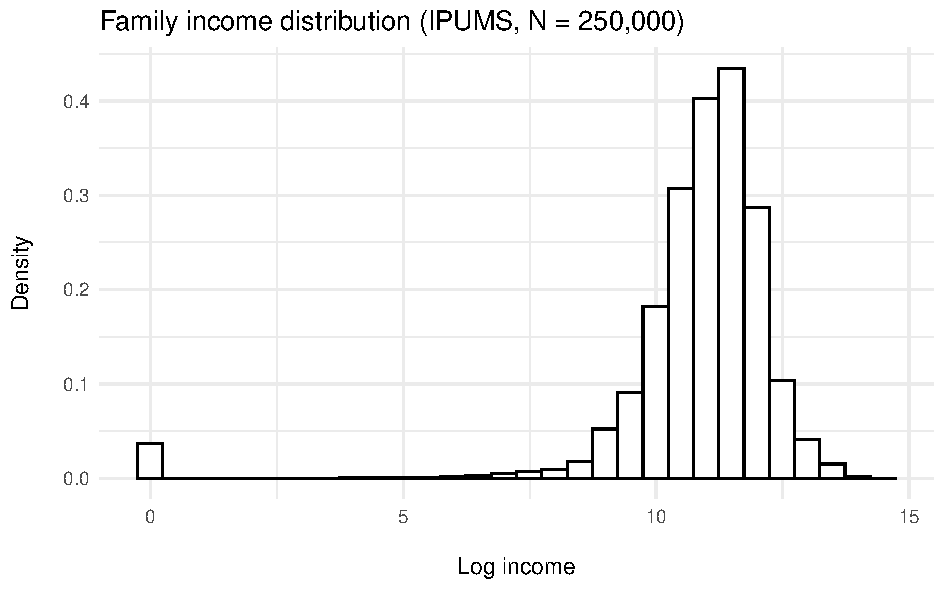
\includegraphics[width=\textwidth]{plots/verification/income/income_ipums.pdf}
     \end{subfigure}
    %  \hfill
     \begin{subfigure}[b]{0.45\textwidth}
         \centering
         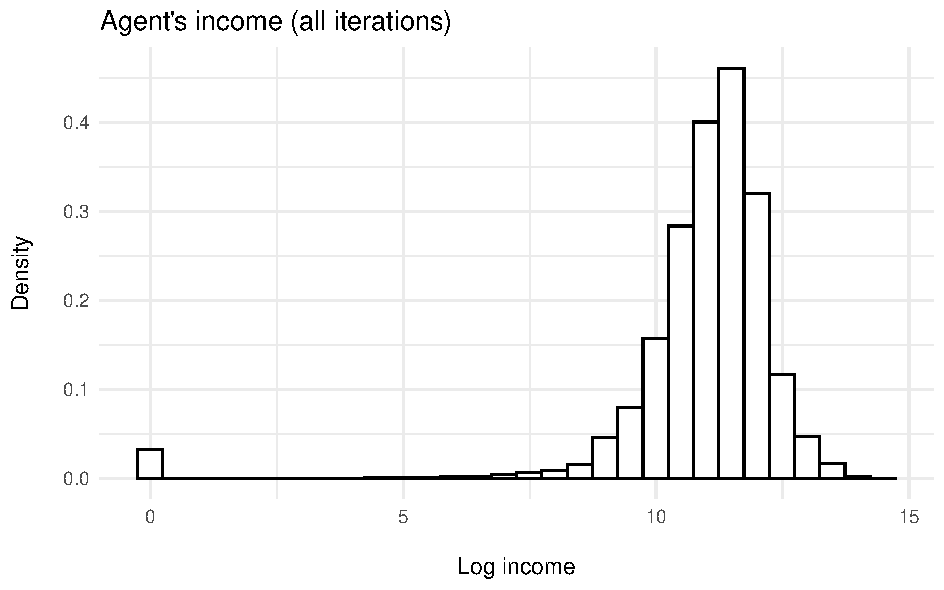
\includegraphics[width=\textwidth]{plots/verification/income/income_mia.pdf}
     \end{subfigure}
\end{figure}


The transition matrices shown below correspond to the average transition probabilities across agents and replicates for each of the three scenarios we explored. The first matrix $I_1$ displays the expected probabilities and they are pretty close to the expected values: 0.30 for the diagonal and 0.175 elsewhere. The overall rank-rank slope in this iteration is 0.13 (all agents), almost the same as the average of county's rank-rank slopes (0.12, SD = 0.08), while the NSI is 0.35 (see Table \ref{ch04:verification_income_stats}). 

\begin{center}
\begin{equation*}
\footnotesize
\label{ch04:verification_trans_mob}
\begin{aligned}
    I_1 = 
% latex table generated in R 4.0.2 by xtable 1.8-4 package
% Tue Jan 05 12:20:36 2021
\begin{bmatrix}{}
  0.299 & 0.175 & 0.176 & 0.175 & 0.175 \\ 
  0.176 & 0.300 & 0.175 & 0.175 & 0.175 \\ 
  0.175 & 0.175 & 0.300 & 0.175 & 0.175 \\ 
  0.175 & 0.175 & 0.175 & 0.301 & 0.174 \\ 
  0.175 & 0.175 & 0.175 & 0.175 & 0.301 \\ 
  \end{bmatrix}

\end{aligned}
\qquad \qquad
\begin{aligned}
  I_2 = 
% latex table generated in R 4.0.2 by xtable 1.8-4 package
% Tue Jan 05 12:20:39 2021
\begin{bmatrix}{}
  0.331 & 0.165 & 0.163 & 0.168 & 0.173 \\ 
  0.161 & 0.333 & 0.166 & 0.168 & 0.172 \\ 
  0.159 & 0.163 & 0.342 & 0.170 & 0.166 \\ 
  0.160 & 0.163 & 0.168 & 0.343 & 0.166 \\ 
  0.160 & 0.166 & 0.161 & 0.162 & 0.351 \\ 
  \end{bmatrix}

\end{aligned}
\end{equation*}
\end{center}

\begin{center}
\begin{equation*}
\footnotesize
\begin{aligned}
    I_3 = 
% latex table generated in R 4.0.2 by xtable 1.8-4 package
% Tue Jan 05 12:05:15 2021
\begin{bmatrix}{}
  0.322 & 0.263 & 0.190 & 0.134 & 0.091 \\ 
  0.222 & 0.234 & 0.216 & 0.192 & 0.137 \\ 
  0.151 & 0.186 & 0.215 & 0.235 & 0.213 \\ 
  0.112 & 0.149 & 0.199 & 0.259 & 0.281 \\ 
  0.096 & 0.112 & 0.170 & 0.247 & 0.376 \\ 
  \end{bmatrix}

\end{aligned}
\end{equation*}
\end{center}


\vspace{5mm}
The second scenario adds the effect of average exposure to income composition on the transition probabilities using $w_k = 0.5$. The probabilities of being in the same income group of their parents (diagonal) increase about 4 percentage points, while county's resources generate more variability in the probabilities outside the diagonal, although differences are not bigger than 1 percentage point. Interestingly, the NSI increases as the probability of being in the same income group of the previous generation is higher. In other words, the NSI might change independently of the parameters of residential mobility and only due to changes in the transition matrix. The overall rank-rank slope increases, while the average of county's rank-rank slopes is closer to 0 with a slightly higher standard deviation (0.06, SD = 0.09). The second scenario generates a higher number of counties with a small or negative rank-rank slope (see Figure \ref{ch04:verification_rank_slope}) as counties become relatively more homogeneous (higher NSI and lower variability of income within counties). 

\vspace{5mm}
\begin{table}[htp]
\setlength{\tabcolsep}{5pt}
\centering
\footnotesize
\caption{Summary statistics income generation verification by scenario (30 replicates)}\
\label{ch04:verification_income_stats}
\begin{tabular}{lcccccc}
  \hline
Scenario & NSI & Gini & Rank-rank slope & County's rank-rank Slope & County's rank-rank Slope SD & Avg. Population \\
  \hline
  1 & 0.35 & 0.47 & 0.13 & 0.12 & 0.08 & 8079.50 \\
    2 & 0.40 & 0.47 & 0.16 & 0.06 & 0.09 & 8097.60 \\
    3 & 0.38 & 0.46 & 0.31 & 0.28 & 0.11 & 7994.60 \\
   \hline
\end{tabular}
\end{table}
\vspace{5mm}


\vspace{5mm}
\newpage
\begin{figure}
    \centering
    \caption{County's rank-rank slope distribution (simulated)}
    \label{ch04:verification_rank_slope}
    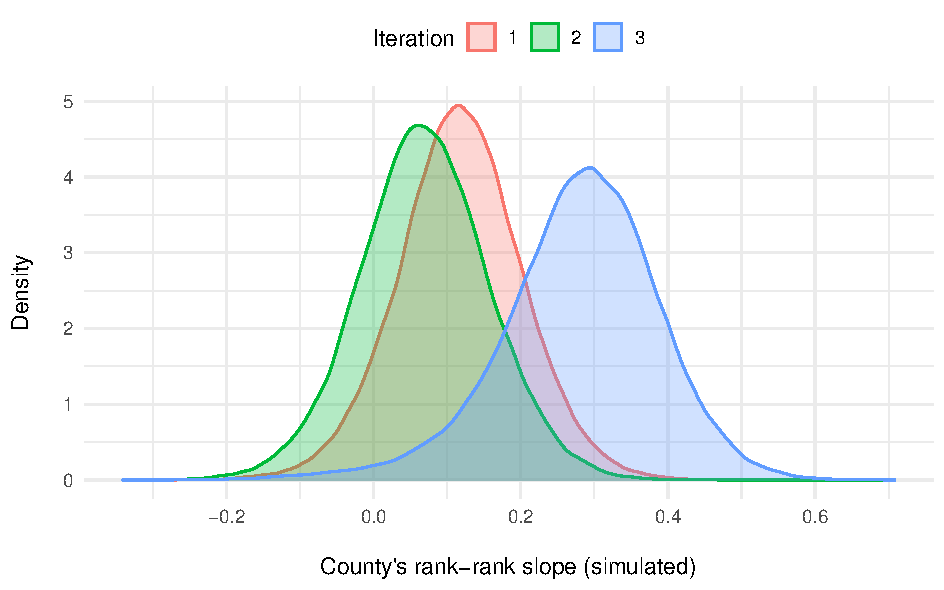
\includegraphics[width=0.7\textwidth]{plots/verification/income/county_rank_slope.pdf}
\end{figure}

Finally, the transition probabilities are defined exogenously by sampling the commuting zone's transition matrices estimated by \citet{chetty2014}. The transition matrix $I_3$ is similar to the overall transition matrix estimated by  \citet{chetty2014} (see Equation \ref{ch04:eq_matrices} in the paper). The NSI is 0.38, and the overall rank-rank slope is slightly higher (0.31) than the the average of county's rank-rank slopes (0.28, SE = 0.11). As the observed rank-rank slope distribution in Figure \ref{ch04:rank_slope_distribution} (in the paper), most of the county's rank-rank slopes are positive (Figure \ref{ch04:verification_rank_slope}). The NSI is similar to the second scenario, but mostly due to an increase in the probability of the transition matrix diagonal for the lowest and the highest quintile rather than a higher overall county homogeneity. Indeed, the standard deviation of the variability of the income distribution within counties is higher than what we observe in iterations one and two.

\subsection{Smoking}

MIA defines the smoking status of agents at age 30 using Equation \ref{ch04:eq_smoking} in the paper. To assess the absolute magnitude of the effect of income mobility on life expectancy, we calibrated the smoking prevalence by income quintile so that the proportion of smokers  matches the proportions observed in NHIS 2019 when the income mobility coefficient $\beta_{s_{imob}}$ is higher than zero. Table \ref{ch04:tab_smoking_distribution} displays the smoking prevalence by income quintile. When $\beta_{s_{imob}}$ is equal to the effect estimated by \citet{daza2021} (MIA treatment), the proportion of smokers increases by 5 percentage points with respect to the counterfactual where $\beta_{s_{imob}}  = 0$. The distribution of the column \textit{MIA treatment} is pretty close to the empirical distribution estimated using NHIS 2019. The effect of smoking on mortality also generates life expectancy differences that are about 10 years on average (10.9). As expected, those differences are practically the same across income groups.

\vspace{5mm}
\begin{table}[htp]
\setlength{\tabcolsep}{15pt}
\centering
\footnotesize
\caption{Proportion smoking by income quintile}
\label{ch04:tab_smoking_distribution}
\begin{threeparttable}
\begin{tabular}{lccc}
  \hline
Income group & NHIS 2019 & MIA Counterfactual & MIA Treatment \\
  \hline
  1 & 0.29 & 0.21 & 0.28 \\
  2 & 0.22 & 0.15 & 0.22 \\
  3 & 0.16 & 0.09 & 0.13 \\
  4 & 0.11 & 0.07 & 0.10 \\
  5 & 0.05 & 0.03 & 0.04 \\
  Total  & 0.17 & 0.10 & 0.15 \\
   \hline
\end{tabular}
\begin{tablenotes}
\footnotesize
\item NHIS 2019 = 10,338 respondents ages 30-50. MIA counterfactual = 8407 agents (30 replicates), MIA treatment = 8226 agents (30 replicates).
\end{tablenotes}
\end{threeparttable}
\end{table}
\vspace{5mm}


\subsection{Measurement}

We verified rank-rank slope, NSI, Gini coefficient, life expectancy were measured correctly by exporting data generated by MIA, and recomputing those statistics using \textit{raw} data outside Anylogic. The measurement of the county's rank-rank slopes and life expectancies was implemented using moving cohorts (i.e., similar to moving averages), so that we have enough data records to estimate these values every $t$ number of years. While Figure \ref{ch04:measurement_diagram} displays how MIA record information at the agent level, Figure \ref{ch04:measurement_verification} shows the size's distribution of the cohorts used to estimate both rank-rank slopes, and life expectancy. 

\newpage
\begin{figure}
    \centering
    \caption{Agent's measurement diagram}
    \label{ch04:measurement_diagram}
    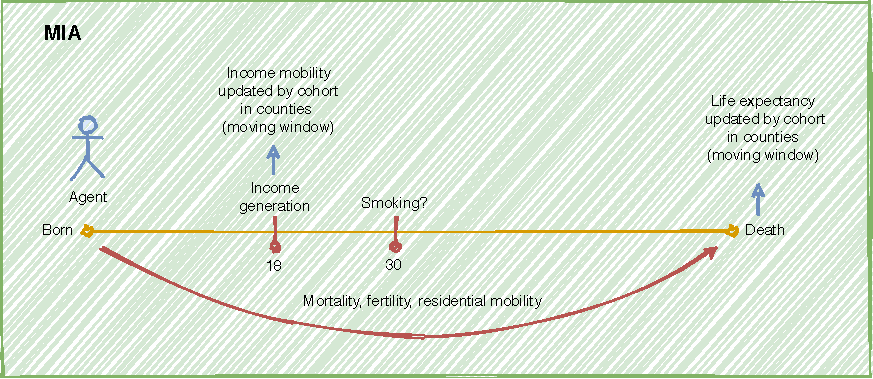
\includegraphics[width=0.7\textwidth]{plots/measurement-diagram.pdf}
\end{figure}

\vspace{5mm}
\begin{figure}[htp]
    \caption{Cohort size to estimate county's rank-rank slope and life expectancy (30 replicates)}\vspace{5mm}
    \label{ch04:measurement_verification}
     \centering
     \begin{subfigure}[b]{0.50\textwidth}
         \centering
         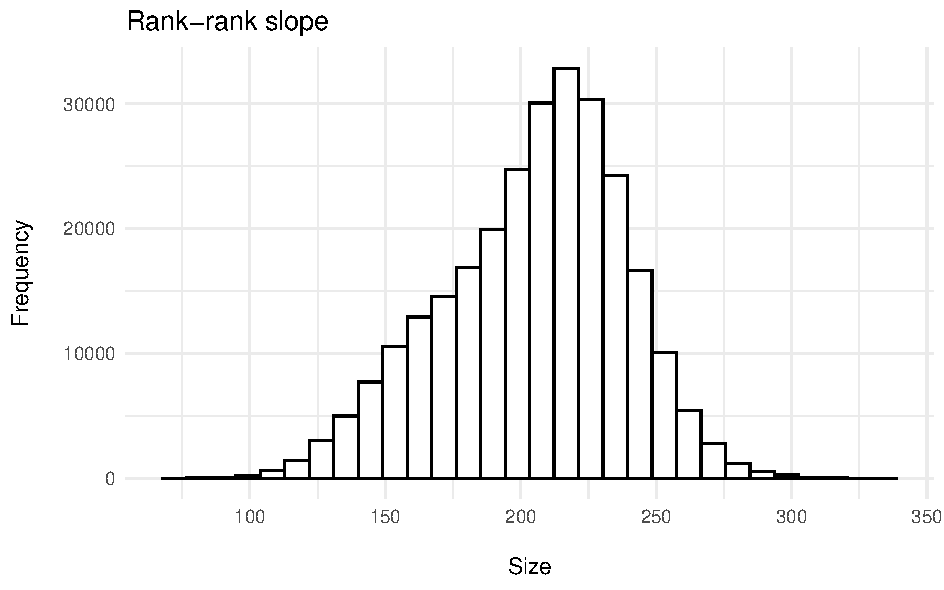
\includegraphics[width=\textwidth]{plots/verification/measurement/im_cohort_size.pdf}
     \end{subfigure}%
     \begin{subfigure}[b]{0.50\textwidth}
         \centering
         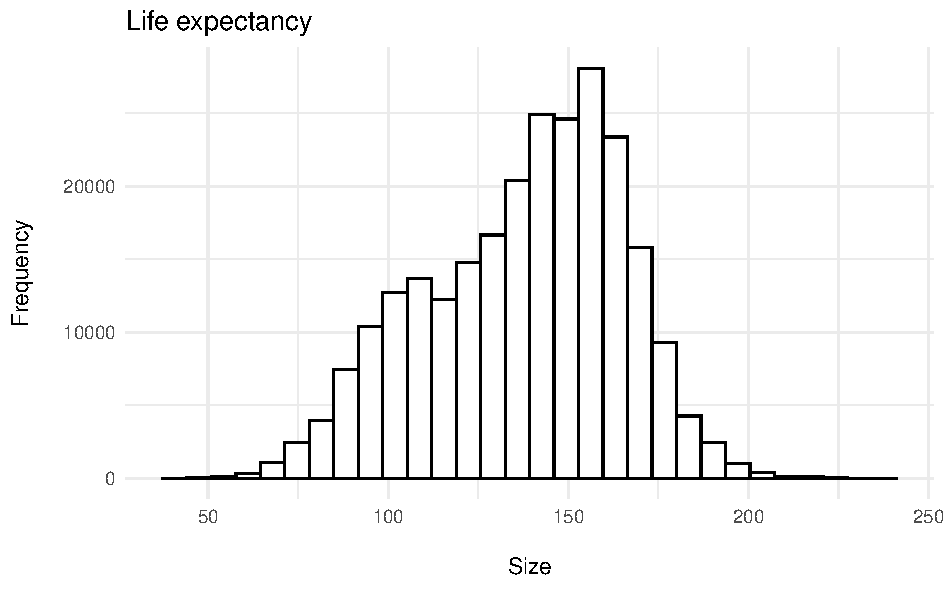
\includegraphics[width=\textwidth]{plots/verification/measurement/mortality_cohort_size.pdf}
     \end{subfigure}\vspace{7mm}
    %  \begin{subfigure}[b]{0.4\textwidth}
    %      \centering
    %      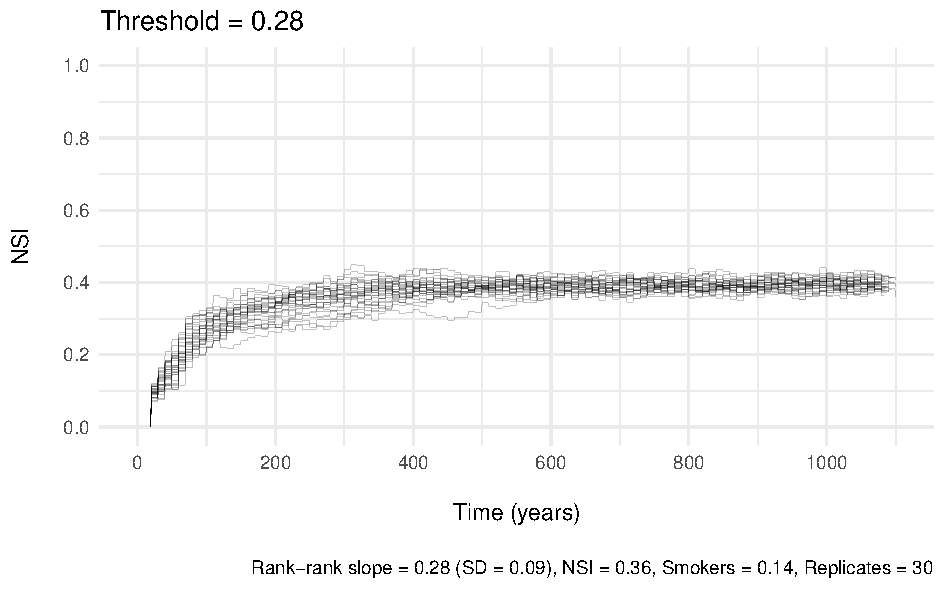
\includegraphics[width=\textwidth]{plots/verification/segregation/nsi_3.pdf}
    %  \end{subfigure}
\end{figure}


\clearpage

\onlyifstandalone{
\singlespacing
\setlength\bibitemsep{5pt}
\printbibliography[title={References}]
\end{refsection}
}

